\section{Combined Lorentz-internal manifolds}
\label{sec:combined}

\subsection{Definition}

Split the eight coordinates of either spacetime into the four of a four-dimensional world,
$x1,x2,x3$ (space) and $x4$ (time), and the four of a fibre, $x0,x5,x6,x7$. The \emph{combined
manifold} is the product $\mathcal M^{3,1}_{\rm NG}\times\mathcal K_{\rm NG}$ of the four-dimensional
Minkowski spacetime $\mathcal M^{3,1}_{\rm NG}$ (coordinates $x1,\dots,x4$) and the fibre
$\mathcal K_{\rm NG}$ (coordinates $x0,x5,x6,x7$), with the metric $\eta_{1671}$ or $\eta_{1644}$
restricted to each factor: on $7+1$ the fibre $\mathcal K^4_{\rm NG}$ is Euclidean, on $4+4$ the fibre
$\mathcal K^{1,3}_{\rm NG}$ has one direction ($x0$) with $\eta_{1644}=+1$ and three ($x5,x6,x7$) with
$\eta_{1644}=-1$. Its tangent space at every point is the same eight-dimensional vector space as
before, but its symmetry is reduced from the eight-dimensional Lorentz group to the product of the
Lorentz group of $\mathcal M^{3,1}_{\rm NG}$ and the rotation group of $\mathcal K_{\rm NG}$. We consider two
readings of the fibre, which Sec.~\ref{sec:renorm} distinguishes sharply: (i) \emph{geometric}: a
compact manifold, for example a torus of radius $R_{\rm NG}$, on which fields may depend (Kaluza and
Klein~\cite{Kaluza1921,Klein1926}); (ii) \emph{internal}: the fields do not depend on $x0,x5,x6,x7$, so the
fibre carries no momentum and its rotations act on the field components only, like an internal
symmetry. Figure~\ref{fig:manifolds} shows the split and its octonionic meaning: on $7+1$ the
four-dimensional world is the algebra of quaternions inside the octonions (time is the real unit) and
the fibre is its complement $\mathbb H_{\rm NG}\mathsf e_4$; on $4+4$ the world is spanned by
$\mathsf e_1,\mathsf e_2,\mathsf e_3,\mathsf e_4$ and the fibre by $\mathsf e_0,\mathsf e_5,\mathsf e_6,\mathsf e_7$.

\begin{figure}[t]
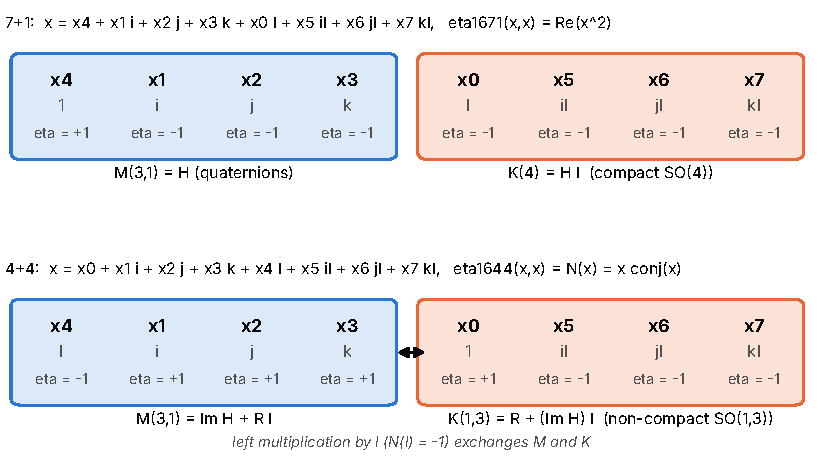
\includegraphics[width=\columnwidth]{../figures/fig_ng_manifolds.pdf}
\caption{The two combined manifolds: the coordinates, the octonion units attached to them, and the
signs of the metric. Blue: the four-dimensional world $\mathcal M^{3,1}_{\rm NG}$; orange: the fibre
$\mathcal K_{\rm NG}$. On $4+4$ the left multiplication by $\mathsf e_4$ (norm $-1$) exchanges the two.}
\label{fig:manifolds}
\end{figure}

\subsection{Lorentz generators become internal generators}

The 28 generators $\Sigma^{AB}_{1671}=\tfrac14[\gamma^A_{1671},\gamma^B_{1671}]$ of the eight-dimensional
Lorentz algebra fall into three sets: the six with $A,B$ both in $\{1,2,3,4\}$ (the Lorentz algebra
$\mathfrak{so}(3,1)$ of the world), the six with $A,B$ both in $\{0,5,6,7\}$ (the rotations of the fibre),
and the 16 mixed ones. The first two sets commute exactly, and every mixed generator fails to commute
with some generator of the first set (check K-1); the same holds for $4+4$. On the combined manifold
only the first two sets remain symmetries, and the second set acts on the fields \emph{at each point of
the world}: from the four-dimensional point of view it is an internal symmetry, although it is a
part of the eight-dimensional Lorentz group. This is the precise sense in which Lorentz degrees of
freedom become internal ones; the conclusion of the Coleman-Mandula theorem holds in four
dimensions (the world's Lorentz algebra and the fibre algebra commute), and in eight dimensions its
hypothesis H1 fails, because the background---the product structure---is not invariant under the
mixed generators.

\emph{Compact on $7+1$, non-compact on $4+4$.} On $7+1$ every generator $2\Sigma^{ab}_{1671}=
\gamma^a_{1671}\gamma^b_{1671}$ of the fibre squares to $-\mathsf 1_{16}$, so its eigenvalues are imaginary;
the trace form of the six generators (the trace of the product of two of them, as a quadratic form on their real combinations) is negative definite, and the fibre
algebra is the compact $\mathfrak{so}(4)$. On $4+4$ the three generators $2\Sigma^{0t}_{1644}$ square to
$+\mathsf 1_{16}$ and the trace form has signature $(3,3)$: the fibre algebra is the non-compact
$\mathfrak{so}(1,3)$ (check K-2). \emph{Theorem 3.} No positive-definite scalar product on the 16
components is invariant under the fibre algebra of $4+4$. \emph{Proof.} If a positive-definite scalar
product were invariant, every generator would be anti-Hermitian with respect to it and would have
purely imaginary eigenvalues; $\Sigma^{05}_{1644}$ has the real eigenvalues $\pm\tfrac12$. $\square$
The eight-dimensionally covariant density shows the same: on $7+1$ the Dirac conjugation matrix
$\mathsf A_{\rm NG}=\gamma^4_{1671}$, defined by $\mathsf A_{\rm NG}\Sigma^{AB}_{1671}\mathsf A_{\rm NG}^{-1}=
-(\Sigma^{AB}_{1671})^\dagger$ for all 28 generators, gives the density $\psi^\dagger_{1671}\mathsf A_{\rm NG}
\gamma^4_{1671}\psi_{1671}=\psi^\dagger_{1671}\psi_{1671}$, positive; on $4+4$ the conjugation matrix is
$\mathsf A_{\rm NG}=\gamma^4_{1644}\gamma^5_{1644}\gamma^6_{1644}\gamma^7_{1644}$ and the density matrix
$\mathsf A_{\rm NG}\gamma^4_{1644}=\gamma^5_{1644}\gamma^6_{1644}\gamma^7_{1644}$ is traceless with square
$\mathsf 1_{16}$, so the density is indefinite and the Fock space has states of negative norm (check K-7).
A theory of the $4+4$ field with positive norm keeps, of the fibre algebra, only its compact form,
spanned by $\Sigma^{st}_{1644}$ and $i\Sigma^{0t}_{1644}$ (Sec.~\ref{sec:superfluid}).

\emph{Spinors.} In statements that hold on both spacetimes, $\gamma^A_{\rm NG}$ denotes the Dirac
matrices of the spacetime under discussion ($\gamma^A_{1671}$ or $\gamma^A_{1644}$), and likewise
$\Sigma^{AB}_{\rm NG}$, $\omega_{\rm NG}$, $C^\pm_{\rm NG}$, $\beta_{\rm NG}$, $\alpha^j_{\rm NG}$ (the matrices
of the project), $\psi_{\rm NG}$ (the field $\psi_{1671}$ or $\psi_{1644}$) and $m_{\rm NG}$ (its mass). The products
$\omega^{\rm 4D}_{\rm NG}=\gamma^1_{\rm NG}\gamma^2_{\rm NG}\gamma^3_{\rm NG}\gamma^4_{\rm NG}$ and
$\omega^{\rm int}_{\rm NG}=\gamma^0_{\rm NG}\gamma^5_{\rm NG}\gamma^6_{\rm NG}\gamma^7_{\rm NG}$ commute; the 16
products of $\gamma^1_{\rm NG},\dots,\gamma^4_{\rm NG}$ and the 16 products of
$\omega^{\rm 4D}_{\rm NG}\gamma^a_{\rm NG}$ are each linearly independent, and the two sets commute, so the 16 components are the tensor product of a
four-dimensional Dirac spinor of the world and a four-component spinor of the fibre (check K-3). On
$7+1$, $(\omega^{\rm int}_{\rm NG})^2=+\mathsf 1_{16}$ splits the fibre spinor into the two real doublets of
$\mathfrak{so}(4)=\mathfrak{su}(2)\oplus\mathfrak{su}(2)$; on $4+4$, $(\omega^{\rm int}_{\rm NG})^2=-\mathsf 1_{16}$ and the
two doublets are complex conjugates, as for the Lorentz group.

\subsection{The octonions lock rotations to internal rotations}

The octonions carry the \emph{associative three-form} $\phi_{\rm NG}(\mathsf x,\mathsf y,\mathsf z)=
\langle\mathsf x,\mathsf y\mathsf z\rangle_{\rm NG}$ on the imaginary units; its symmetry group in the rotations
of the seven imaginary directions is $\mathrm G_2$. Consider, on $7+1$, the rotations of ordinary space
(the imaginary quaternions $\mathsf e_1,\mathsf e_2,\mathsf e_3$, algebra $\mathfrak{so}(3)$) and of the fibre
($\mathsf e_4,\dots,\mathsf e_7$, algebra $\mathfrak{so}(4)$). Inside $\mathfrak{so}(3)\oplus\mathfrak{so}(4)$ (dimension 9)
the elements that leave $\phi_{\rm NG}$ unchanged form an algebra of dimension
{{GEN:g2_stab_full}}; the same algebra leaves unchanged the six components
$\phi_{\rm NG}(\mathsf e_j,\mathsf e_{u_{\rm NG}(a)},\mathsf e_{u_{\rm NG}(b)})$ with one unit of ordinary space and two of the fibre (their part
$\phi^{\rm mix}_{\rm NG}$). It projects \emph{onto} the space rotations (rank
{{GEN:g2_proj_rank}}), contains no rotation of space alone (dimension {{GEN:g2_pure_space}}), and
contains {{GEN:g2_pure_int}} rotations of the fibre alone (checks K-5a, K-5b; Fig.~\ref{fig:locking}).
The same six-dimensional algebra is obtained from the derivations: the elements of
$\mathrm{Der}(\mathbb O_{\rm NG})=\mathfrak g_2$ that preserve the quaternions and their complement (check
K-5c). \emph{Every rotation of space that preserves the octonionic structure is accompanied by a
rotation of the fibre.}

\begin{figure}[t]
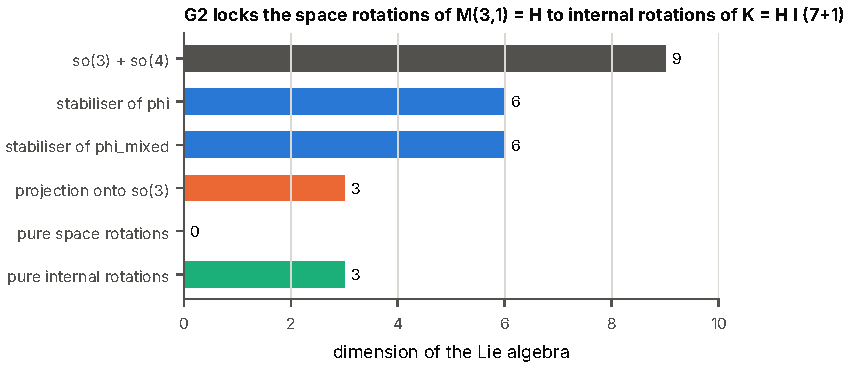
\includegraphics[width=\columnwidth]{../figures/fig_ng_locking.pdf}
\caption{Dimensions of the Lie algebras of the $\mathrm G_2$ locking on $7+1$. Of the nine rotations of
space and fibre, six preserve the associative three-form; they include every rotation of space, but
none without a rotation of the fibre. Data: \texttt{data/ng\_g2\_locking.csv}.}
\label{fig:locking}
\end{figure}

A background with these symmetries is a condensate of the pairs $\psi^T_{1671}C^+_{1671}
\gamma^j_{1671}\gamma^a_{1671}\gamma^b_{1671}\psi_{1671}$, with one space index and two fibre indices, whose
amplitudes are proportional to $\phi_{\rm NG}(\mathsf e_j,\mathsf e_{u_{\rm NG}(a)},\mathsf e_{u_{\rm NG}(b)})$. These
pairs are nonzero but vanish for two particles at rest (they are p-wave pairs, Sec.~\ref{sec:superfluid}),
and the condensate picks a rest frame: it can exist only in a medium, which breaks the boosts
(hypothesis H1). In such a medium the unbroken rotations are the diagonal combinations of space and
fibre rotations---the octonionic analogue of the B phase of superfluid helium-3, where the
condensate locks spin to orbital rotations~\cite{BalianWerthamer1963,Leggett1975}, of the
colour-flavour locking of dense quark matter~\cite{AlfordRajagopalWilczek1999}, and of the
``spin from isospin'' of Refs.~\cite{JackiwRebbi1976,HasenfratzTHooft1976}.

\subsection{Split octonions exchange space-time and fibre}

On $4+4$ the left multiplication $L_{\rm NG}(\mathsf e_4)$ by the split unit $\mathsf e_4$, of norm $-1$, is an
\emph{anti-isometry}: $N_{\rm NG}(\mathsf e_4\mathsf x)=-N_{\rm NG}(\mathsf x)$, and $L_{\rm NG}(\mathsf e_4)^2=\mathsf 1_8$.
It maps $\mathsf e_1,\mathsf e_2,\mathsf e_3,\mathsf e_4$ (the world) onto $\pm\mathsf e_5,\pm\mathsf e_6,\pm\mathsf e_7,
\mathsf e_0$ (the fibre) and back, and conjugation by it maps the Lorentz algebra $\mathfrak{so}(3,1)$ of the
world onto the algebra $\mathfrak{so}(1,3)$ of the fibre and back (check K-6). Since the overall sign of
a metric is a convention, the split-octonion product makes the distinction between space-time and
internal directions of $4+4$ a matter of choice; together with triality (Sec.~\ref{sec:triality}),
which permutes vectors and spinors, even the distinction between space-time vectors and spinors is
not invariant. On $7+1$ no such exchange exists: the Lorentz algebra of the world, with trace form of
signature $(3,3)$, is not isomorphic to the compact fibre algebra (check K-2).

\subsection{Mass splitting and the Kaluza-Klein spectrum}

\emph{O'Raifeartaigh.} A rotation of $7+1$ in the plane of $x1$ and $x0$ with cosine $\tfrac35$ and
sine $\tfrac45$ is an element of the eight-dimensional Poincar\'e group, which is finite-dimensional
and contains the four-dimensional one. Applied to a momentum with time component 5 and $x1$
component 3, it keeps the eight-dimensional mass squared 16 but changes the four-dimensional mass
squared $(5)^2-(\text{space part})^2$ from 16 to $\tfrac{544}{25}$ (exact, check K-8). There is no
contradiction with the theorem: a single eight-dimensional particle has a continuous spectrum of
four-dimensional masses, from its eight-dimensional mass upwards, so hypothesis H7 fails.

\emph{Kaluza-Klein modes.} On a torus fibre of radius $R_{\rm NG}$ a field of mass $m_{\rm NG}$ (the
mass $m_{1671}$ or $m_{1644}$ of the field of the spacetime under discussion) has the modes
$\exp(i\sum_a n^a_{\rm NG}x^a/R_{\rm NG})$ with integers $n^a_{\rm NG}$. Squaring the Dirac equation
$(i\gamma^A_{1671}\partial_A-m_{1671})\psi_{1671}=0$ of $7+1$ gives $(\eta^{AB}_{1671}\partial_A\partial_B+
m_{1671}^2)\psi_{1671}=0$, and squaring the Dirac equation $(\gamma^A_{1644}\partial_A-m_{1644})\psi_{1644}=0$
of $4+4$ gives $(\eta^{AB}_{1644}\partial_A\partial_B-m_{1644}^2)\psi_{1644}=0$. Inserting a mode with energy
$\varepsilon_{\rm NG}$ and momentum $\vec q$ in the world gives $\varepsilon_{\rm NG}^2=q^2+(m^{\rm eff}_{\rm NG})^2$ with
the four-dimensional mass squared
\begin{align}
(m^{\rm eff}_{\rm NG})^2&=m_{1671}^2+\textstyle\sum_a(n^a_{\rm NG})^2/R_{\rm NG}^2\quad(7{+}1),\nonumber\\
(m^{\rm eff}_{\rm NG})^2&=m_{1644}^2+\big[(n^0_{\rm NG})^2-\textstyle\sum_t(n^t_{\rm NG})^2\big]/R_{\rm NG}^2\quad(4{+}4).
\label{eq:kkmass}
\end{align}
On $7+1$ it is never negative; on $4+4$ it is negative for most modes: a tower of tachyons. With $(m_{\rm NG}R_{\rm NG})^2=1$
and $\lvert n^a_{\rm NG}\rvert\le n^{\max}_{\rm NG}=12$ the tachyonic fraction is {{GEN:kk_tach_fraction}} (check K-9,
Fig.~\ref{fig:kk}). A geometric $4+4$ fibre is therefore inconsistent: the $4+4$ combined manifold
admits only the internal reading, in which the fibre carries no momentum.

\begin{figure*}[t]
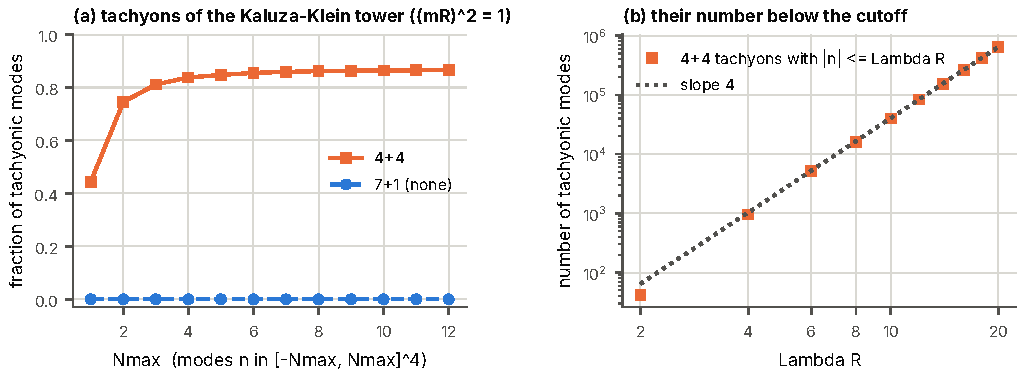
\includegraphics[width=0.92\textwidth]{../figures/fig_ng_kk.pdf}
\caption{Kaluza-Klein modes on a torus fibre with $(m_{\rm NG}R_{\rm NG})^2=1$. (a) Fraction of tachyonic
modes among all modes with $\lvert n^a_{\rm NG}\rvert\le n^{\max}_{\rm NG}$ (Nmax in the figure): none on $7+1$,
most of them on $4+4$.
(b) The number of $4+4$ tachyons with $\sum_a(n^a_{\rm NG})^2\le(\Lambda_{\rm NG}R_{\rm NG})^2$ grows like
$(\Lambda_{\rm NG}R_{\rm NG})^4$. Data: \texttt{data/ng\_kk\_tachyons.csv},
\texttt{data/ng\_kk\_tachyons\_cutoff.csv}.}
\label{fig:kk}
\end{figure*}
